\documentclass[12pt,a4paper]{article}
\usepackage[utf8]{inputenc}
\usepackage[brazil]{babel}
\usepackage[left=3cm,right=3cm,top=2.5cm,bottom=2.5cm]{geometry}
\usepackage{setspace}
\usepackage{amsmath, mathrsfs, amssymb, mathtools}
\usepackage{amsthm}
\usepackage{multirow}
\usepackage{hyperref}
\usepackage{listings}
\usepackage{graphicx}
\graphicspath{{./imagens/}}


% Custom colors
\usepackage{xcolor}

\definecolor{codegreen}{rgb}{0,0.6,0}
\definecolor{codegray}{rgb}{0.5,0.5,0.5}
\definecolor{codepurple}{rgb}{0.58,0,0.82}
\definecolor{backcolour}{rgb}{0.95,0.95,0.92}

% Python style for highlighting
\newcommand\pythonstyle{\lstset{
    language=Python,
    backgroundcolor=\color{backcolour},   
    commentstyle=\color{codegreen},
    keywordstyle=\color{magenta},
    numberstyle=\tiny\color{codegray},
    stringstyle=\color{codepurple},
    basicstyle=\ttfamily\footnotesize,
    breakatwhitespace=false,         
    breaklines=true,                 
    captionpos=b,                    
    keepspaces=true,                 
    numbers=left,                    
    numbersep=5pt,                  
    showspaces=false,                
    showstringspaces=false,
    showtabs=false,                  
    tabsize=2
}}

% Python environment
\lstnewenvironment{python}[1][]
{
\pythonstyle
\lstset{#1}
}
{}

% Python for external files
\newcommand\pythonexternal[2][]{{
\pythonstyle
\lstinputlisting[#1]{#2}}}

% Python for inline
\newcommand\pythoninline[1]{{\pythonstyle\lstinline!#1!}}

\sloppy

\title{Processamento Digital de Imagens – Trabalho 2\\Filtros passa-baixa e passa-alta Butterworth}
\author{Guilherme L. Salomão, João Victor M. Freire, \\Martin Heckmann, Renan D. Pasquantonio }
\date{8 de Outubro de 2020}

\begin{document}

\maketitle

\section{Introdução}
A Transformada de Fourier é uma poderosa ferramenta no Processamento Digital de Imagens e Sinais, uma vez que ela permite representar uma imagem (domínio espacial) no domínio das frequências. Essa representação é, em muitos casos, mais simples e intuitiva que a do domínio espacial.

Além de realizar filtragens no domínio da frequência e depois converter a imagem para o domínio espacial novamente, podemos utilizar o Teorema da Convolução para calcular a convolução de uma imagem por um filtro usando Transformadas de Fourier, e depois usando o cálculo da Transformada Inversa, da seguinte forma:
$$
 f(x) * g(x) = \mathscr{F}^{-1}\{F(\mu)G(\mu)\},
$$
na qual $F$ e $G$ são as transformadas de $f$ e $g$, respectivamente, e $\mathscr{F}^{-1}$ é a transformada inversa de Fourier.

Esse teorema nos permite aplicar qualquer filtro linear em uma imagem através da multiplicação das transformadas da imagem e do filtro. Dependendo do tamanho dos filtros que utilizarmos, esse método de filtragem é bem mais eficiente que a convolução e correlação-cruza comum.

\section{Motivação}
Dentre os diversos filtros que existem no domínio da frequência, dois que temos um interesse particular são os filtros passa-baixa e passa-alta.

Como o nome sugere, o filtro passa-baixa permite apenas a passagem de frequências baixas, causando a eliminação de frequências mais altas que são comumente associadas a detalhes de uma imagem. Assim, temos um efeito análogo aos de um filtro de suavização do domínio espacial.

De forma semelhante, o passa-alta elimina frequências menores, e obtém um efeito similar ao cálculo da derivada da imagem.

São diversos os filtros de passa-baixa e passa-alta. Em aula, fomos apresentados ao filtro passa-baixa ideal e gaussiano, e ao passa-alta gaussiano e laplaciano. Além desses, existem também os filtros Butterworth tanto de baixa como de alta. Esses são notáveis por buscarem uma resposta de frequência o mais plana possível, mas sem ser abrupto como no filtro ideal.

\newpage

\section{Explicação do Método Implementado}
\subsection{Passa-Baixa}
A função que vamos utilizar para definir o filtro é:
$$
H(\mu, \nu) = \frac{1}{1 + {\frac{D(\mu, \nu)}{D_0}}^{2n}},
$$
na qual $D(\mu, \nu) = \sqrt{\mu^2 + \nu^2}$. Os valores $D_0$ e $n$ são parâmetros variáveis, e faremos uma análise dos seus efeitos na \hyperref[sec:4]{Seção 4} do documento. A seguir está nossa implementação do filtro:
\pythonexternal{./src/passa_baixa_butterworth.py}

\[FAZER\]

\subsection{Passa-Alta}

\[FAZER\]



\newpage

\section{Análise dos Parâmetros do Filtro}
\label{sec:4}
Os filtros Butterworth recebem dois parâmetros: $D_0$ e $n$. Testamos diferentes valores de cada um para analisarmos como eles afetam o filtro resultante. Fizemos os experimentos com os valores $D_0 = \{0,01; 0,05; 0,10\}$ e de $n = \{1, 3, 5\}$. 

Para esses valores, obtivemos os seguintes filtros passa-baixa:

\vspace{1em}
\begin{center}
	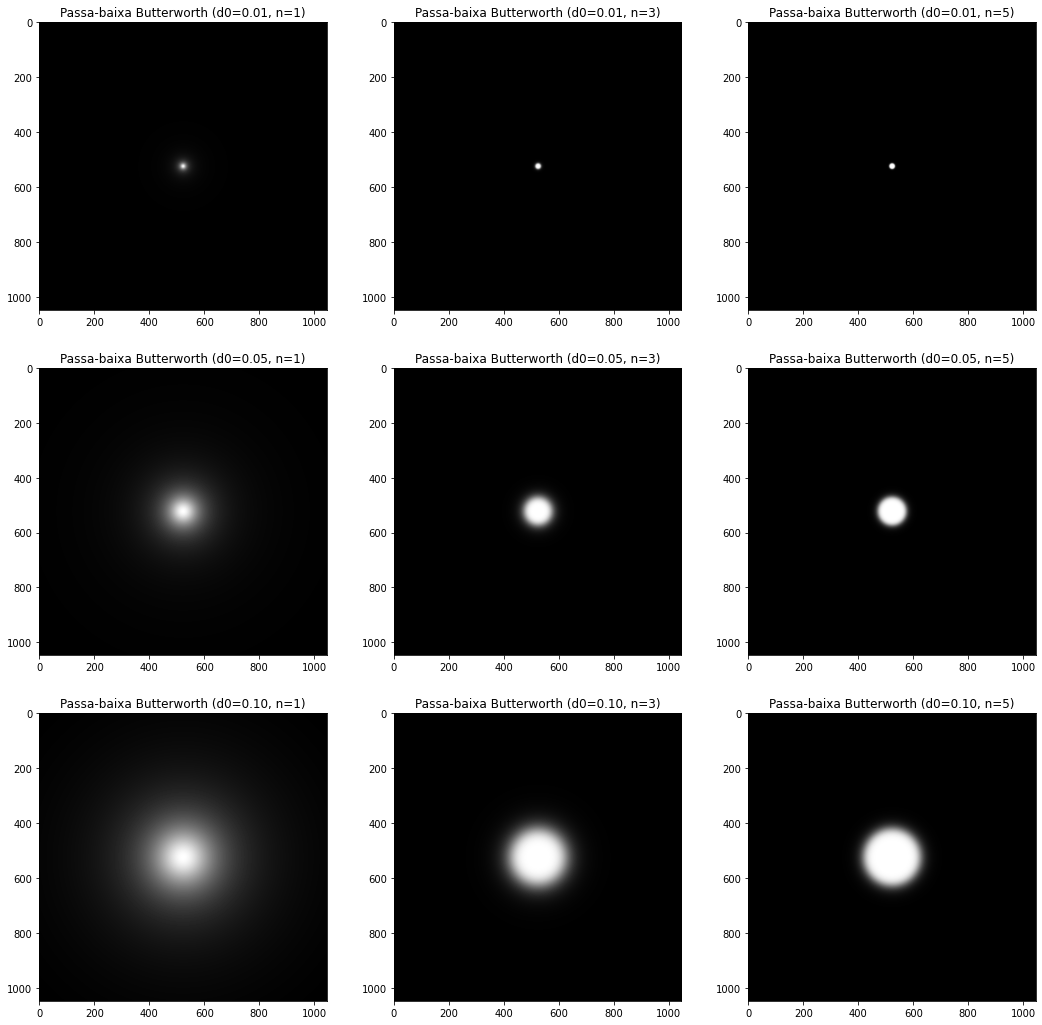
\includegraphics[width=\textwidth]{filtros_low_pass}
\end{center}
\vspace{1em}

Observando os filtros, ficou claro que conforme $D_0$ cresce, o raio das frequências permitidas também cresce. Assim, um valor pequeno de $D_0$ vai fazer uma suavização maior da imagem. Já ao observarmos o parâmetro $n$, percebe-se que que seu valor esta associado com a suavidade da transição entre as frequências permitidas, de forma que um valor grande de $n$ se aproxima de um filtro passa-baixa ideal. A seguir, aplicamos os filtros a uma imagem.

\vspace{1em}
\begin{center}
	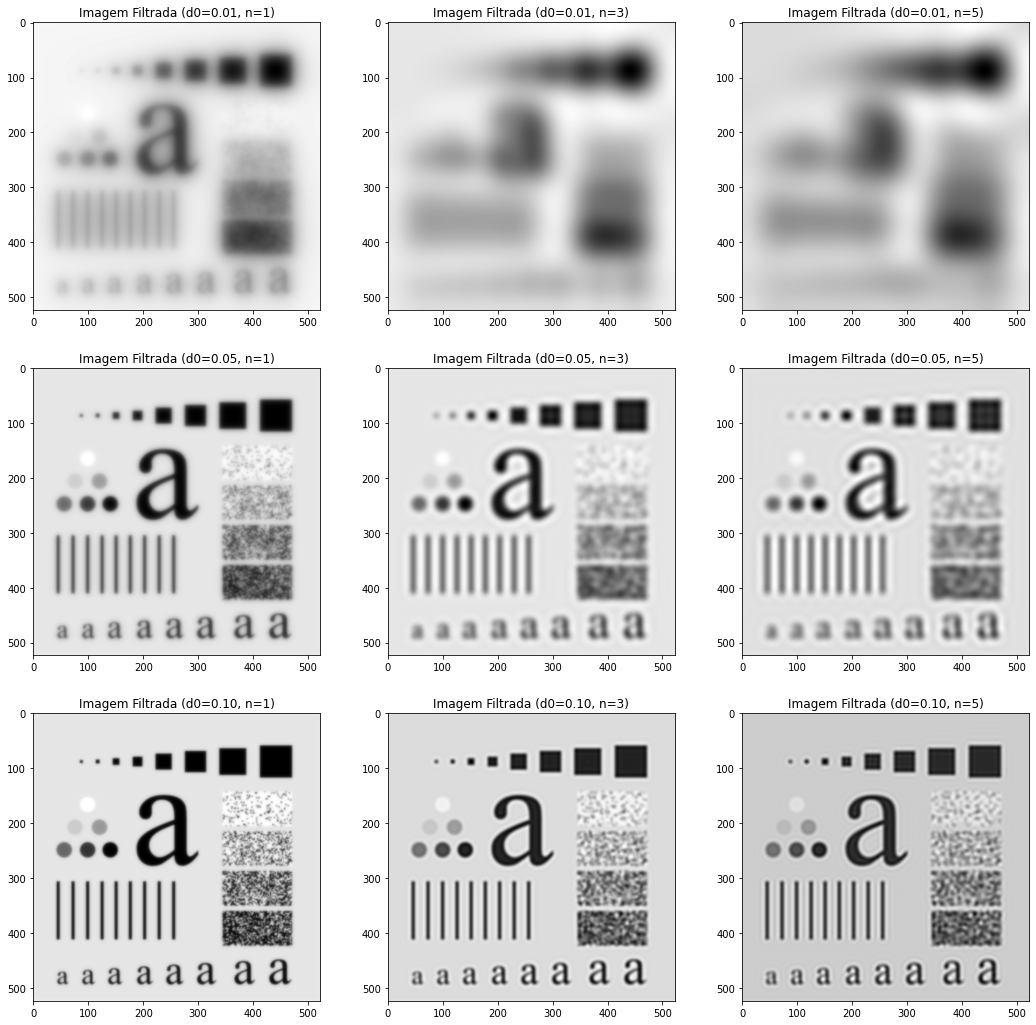
\includegraphics[width=\textwidth]{imagens_low_pass}
\end{center}
\vspace{1em}

Nota-se que, conforme o valor de $n$ cresce e nosso filtro fica mais abrupto, os artefatos de ondulação percebidos no filtro passa-baixa ideal também acontecem aqui. É possível confirmar que o valor de $D_0$ controla o nível da suavização, sendo bastante intensa nos casos em que seu valor é muito pequeno.

Efeitos análogos acontecem no filtro passa-alta. O parâmetro $n$ continua no mesmo lugar, portanto têm o mesmo efeito de controlar a suavidade da transição entre as frequências permitidas e eliminadas. Já a razão que continha $D_0$, $\frac{D(\mu,\nu)}{D_0}$, se tornou $\frac{D_0}{D(\mu,\nu)}$. Assim, $D_0$ passou a controlar o raio das frequências que serão eliminadas.

\vspace{1em}
\begin{center}
	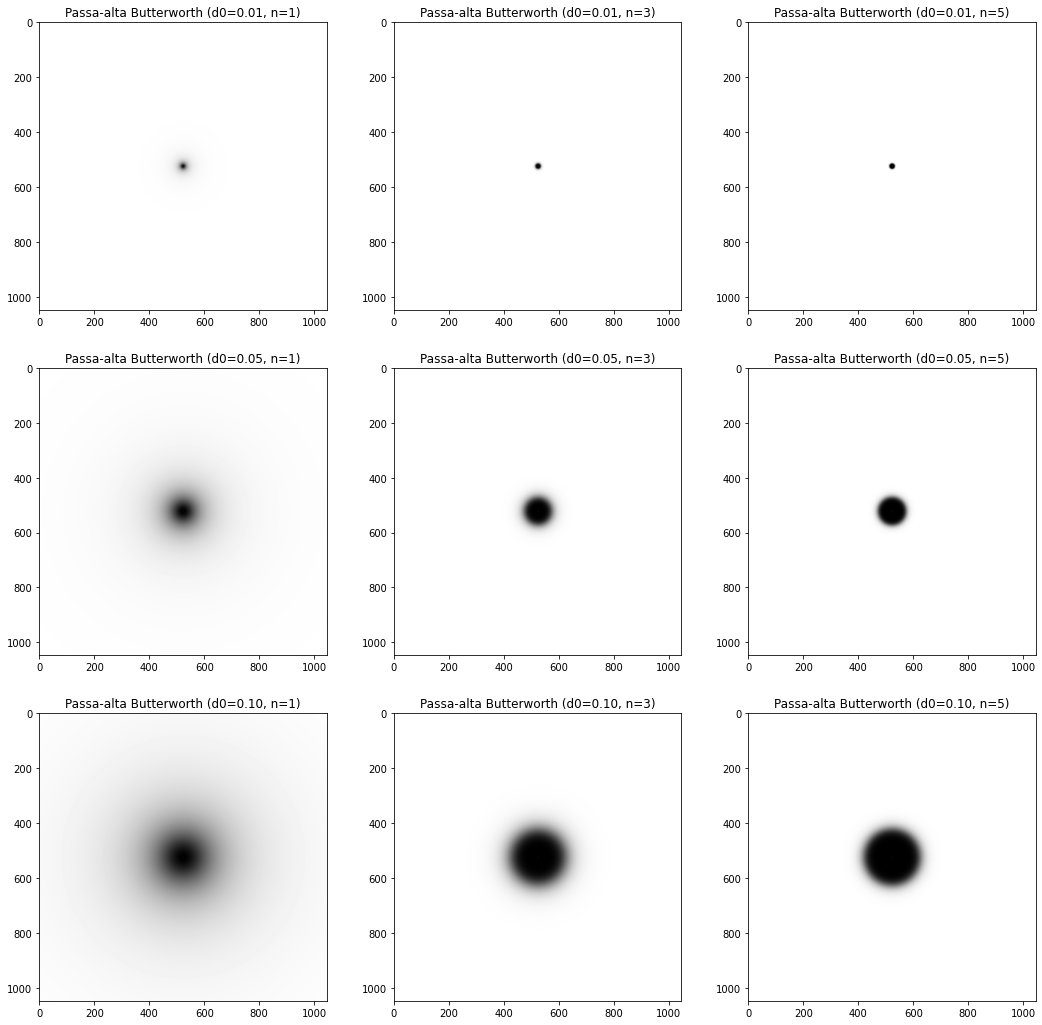
\includegraphics[width=\textwidth]{filtros_high_pass}
\end{center}
\vspace{1em}

Já ao analisarmos as imagens com o filtro aplicado, percebemos que 

\[FAZER\]

Assim sendo, chegamos à conclusão que a melhor forma de escolher os valores de $D_0$ e $n$.

\[FAZER\]

\vspace{1em}
\begin{center}
	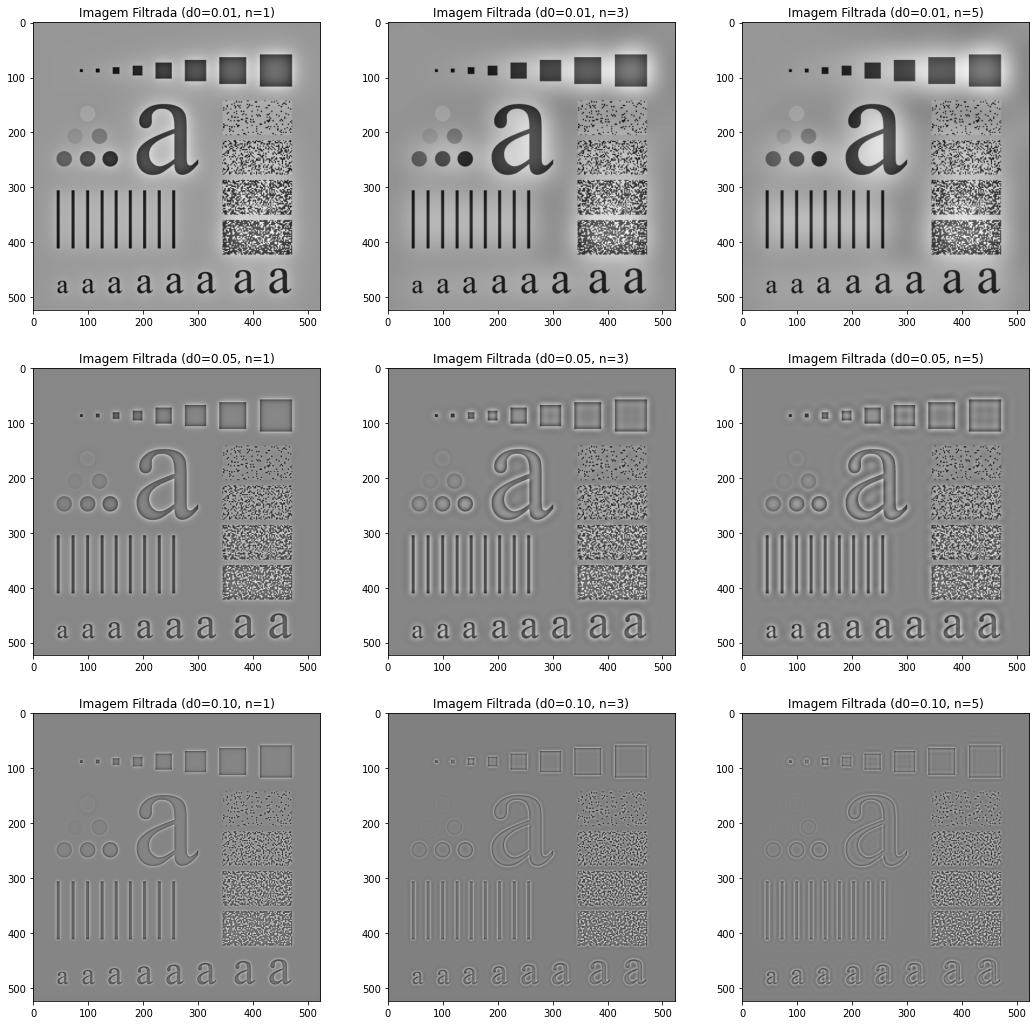
\includegraphics[width=\textwidth]{imagens_high_pass}
\end{center}
\vspace{1em}

\newpage

\nocite{comin2020}
\nocite{wiki01}

\bibliographystyle{acm}
\bibliography{references}

\end{document}
